\section{Resultados e discussão}

Para encontrar todos os resultados necessários para comprovar a teoria, a prática foi dividida em algumas etapas, sendo elas:


\begin{itemize}

    \item Inicialmente foi montado o circuito da figura \ref{ckt:1} substituindo o controle não linear do ganho por um potenciômetro de $50k\ohm$, ajustando-o de tal forma que tentasse garantir uma senoide de 1V de pico na saída do circuito;
    
    \item Medir a resistência do potenciômetro que garante o circuito no limiar de sustentação de oscilações;
    
    \item Por fim o controle não linear foi reposto no lugar do potenciômetro e a forma de onda e a frequência do sinal de saída foi verificado.  
\end{itemize}

Antes de montar o circuito, os valores máximo e mínimo de resistência do potenciômetro foi medida, encontrando uma valor máximo de $52.28k\ohm$ e um valor mínimo de $10.74\ohm$.

Ao tentar ajustar o potenciômetro de forma a garantir uma senoide de 1V de pico, observou-se a impossibilidade de obter tal forma de onda, como já esperada pelas relações \ref{mai} e \ref{men} obtidas na análise teórica.

Ao aumentar muito a resistência do potenciômetro observou-se que a forma de onda saturava-se, indicando instabilidade nos polos da função de transferência de malha fechada (figura \ref{fig:1}). Enquanto que ao diminuir a resistência do potenciômetro, chegava-se a um ponto em que as oscilações não se sustentavam devido à existência de oscilações amortecidas (figura \ref{fig:2}). O valor de resistência ajustado no potenciômetro que garantiu oscilações sustentadas foi cerca de $19.552k\ohm$, cerca do dobro do valor de resistência do resistor $R_1$ da figura \ref{ckt:1} (figura \ref{fig:3}) e com frequência de 996Hz, próxima do valor teórico encontrado em \ref{freqq}. 

\begin{figure}[H] 
\centering
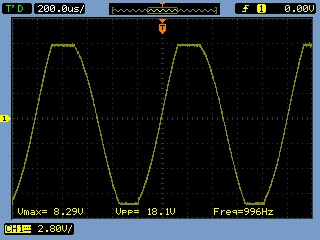
\includegraphics[width=7cm]{images/sat.png}
\caption{Oscilações instáveis. Observa-se que a forma de onda está sendo deformada pela saturação.}
\label{fig:1} 
\end{figure}

\begin{figure}[H] 
\centering
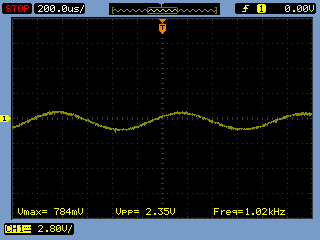
\includegraphics[width=7cm]{images/not.png}
\caption{Oscilações amortecidas. A senoide que antes existia foi totalmente amortecida (observa-se nas medições do osciloscópio a medição da amplitude da senoide que instantes infinitesimais atrás estava ali).}
\label{fig:2} 
\end{figure}


\begin{figure}[H] 
\centering
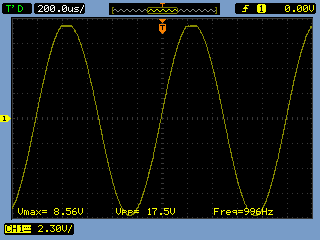
\includegraphics[width=7cm]{images/pot.png}
\caption{Senoide sustentada.}
\label{fig:3} 
\end{figure}

Com o controle não linear do ganho posto no lugar do potenciômetro e trocando $R_2$ do circuito da figura \ref{ckt:1} por um resistor de valor de $100k\ohm$, observou-se a forma de onda da figura \ref{fig:4}.

\begin{figure}[H] 
\centering
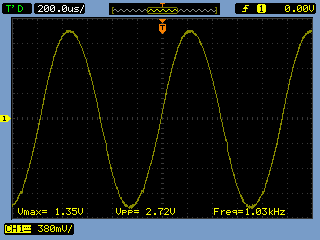
\includegraphics[width=7cm]{images/100k.png}
\caption{Oscilador operando com controle não linear do ganho.}
\label{fig:4} 
\end{figure}

Observa-se que a amplitude não é como a esperada na prática, sendo a amplitude pico-a-pico encontrada de 2.72V e a teórica de 2.1V. Isso se deve, pois na teoria é considerado que a queda de tensão sobre os diodos é de 0.7V, enquanto que na prática esse valor pode variar. 

A estratégia utilizada para alterar o resistor de $47k\ohm$ por um de $100k\ohm$ foi observando que o paralelo de uma resistência série do resistor $R_2$ com os diodos e o resistor $R_3$ deve gerar uma resistência duas vezes maior que a do resistor $R_1$, ou seja $20k\ohm$ para garantir o critério de Barkhausen. Dessa forma encontra-se que a resistência série, antes mencionada deve ser de $220k\ohm$. 

Considerando-se a equação da corrente do diodo \ref{diodo} com a tensão térmica de $V_t = 26mV$, a corrente de saturação $I_S = 1.25 \times 10^{-14}A$ e tensão de operação do diodo em cerca de $V_D = 0.5V$.

\begin{equation} \label{diodo}
I_D = I_S(e^{\frac{V_D}{V_t}}-1) = 2.81 \mu A
\end{equation}

Logo a resistência de um diodo polarizado diretamente será:

\begin{equation} \label{diodo}
R_D = \frac{V_D}{I_D} = 177k\ohm
\end{equation}

Assim para garantir o critério de Barkhausen associou-se o diodo com um resistor de $100k\ohm$.

Aproximando a tensão do diodo para cerca de 0.7V obtém-se uma corrente de $6.15mA$ e uma resistência de $113k\ohm$, implicando em uma diferença significativa, devido a influência da exponencial.
%\newpage